\documentclass{article}
\usepackage{vub}
\usepackage[utf8]{inputenc}
\usepackage[dutch]{babel}
\usepackage{xcolor}
\usepackage{array}
\usepackage{graphicx}
\usepackage{tabularx}
\title{Programmeerproject 2}
\subtitle{Handleiding}
\definecolor{myblueish}{rgb}{0.36, 0.54, 0.66}
\faculty{Sciences and Bio-Engineering Sciences}
\author{Gérard Lichtert\\
        \textcolor{blue}{gerard.Lichtert@vub.be}\\
        \textcolor{myblueish}{0557513}}
\date{\today}
\begin{document}
\maketitle
\tableofcontents
\pagebreak
\section{Opstarten}
Om het programma op te starten: Run eerst main-infrabel.rkt op de computer waar de server op moet staan. 
Dit bestand is te vinden in de "mains" folder. In dit voorbeeld zal dit de Raspberry Pi zijn die gebruikt is voor dit project.
Wanneer main-infrabel.rkt opgestart is zal het wachten voor een verbinding met een client of NMBS. Bij het runnen 
van infrabel zal er wel gespecifieerd moeten worden of dit op de hardware of simulator is.
Om dit te doen moeten we \#t of \#f meegeven als argument. \#t voor hardware en \#f voor de simulator. 
\begin{figure}[h]
    \centering
    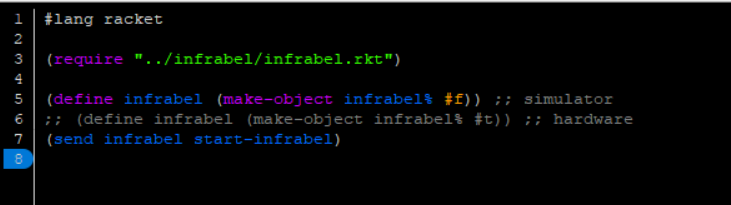
\includegraphics[width=\textwidth]{Images/Screenshot_2.png}
    \caption{Hardware of software definieren.}
\end{figure}
Om de verbinding aan te vragen moeten we main-nmbs.rkt runnen op de andere computer.
Vooraleer we dit doen moeten we wel het adres van de server invoeren. Om dit op te vragen op de Raspberry Pi moeten we
"curl ifconfig.me`` in de terminal typen. Hetgeen dat teruggegeven wordt is het IP adres van de server.
\begin{figure}[h]
    \centering
    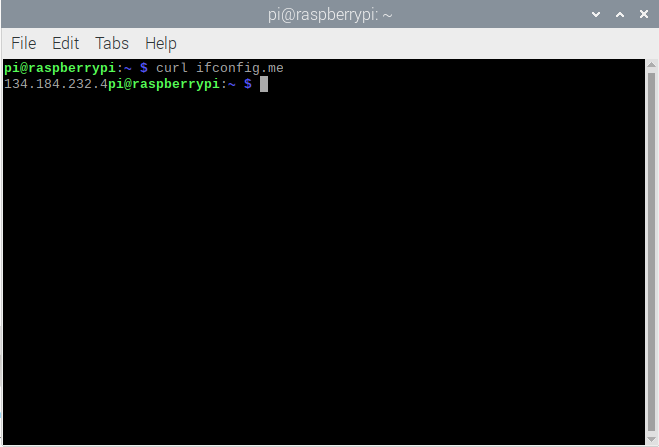
\includegraphics[width=\textwidth, height=8.5cm]{Images/Screenshot from 2021-05-14 05-33-24.png}
    \caption{IP adres opvragen.}
\end{figure}
\\
Om vervolgens het NMBS-component openen. Dit heet main-nmbs.rkt en is te vinden in de "mains" folder. 
Voor dat we het bestand runnen moeten we het opgevraagde ip adres van de server invullen als argument.\\
\begin{figure}[h]
    \centering
    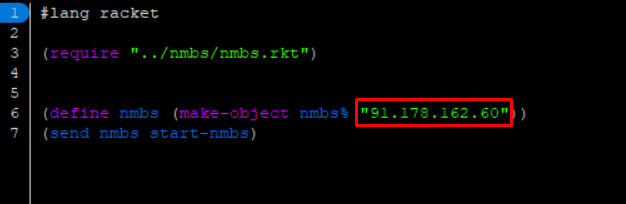
\includegraphics[width=\textwidth]{Images/Screenshot_1.png}
    \caption{Invullen van het IP adres van de server.}
\end{figure}
\\
Hierna kunnen we het bestand runnen. Wanneer we het programma runnen zal er een dialog box opkomen die zal vragen 
op welke manier we het spoornetwerk willen initialiseren. Indien dit op de hardware is zal er maar één optie zijn en als het op
de simulator is zullen er meerdere opties zijn. 
\begin{figure}[h]
    \centering
    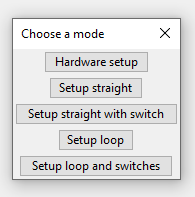
\includegraphics{Images/Screenshot_3.png}
    \caption{Simulator opties.}
\end{figure}
\section{Tabbladen}
\subsection{Menu}
Hier kunnen we de verbinding verbreken met het Infrabel component. Dit is ook de enige optie hier
\subsection{Main}
Dit is de hoofd tabblad waar de meeste interacties mee zullen gebeuren. Nadat er een locomotief is toegevoegd op 
het spoornetwerk kunnen we interageren met de locomotief.
\begin{figure}[h]
    \centering
    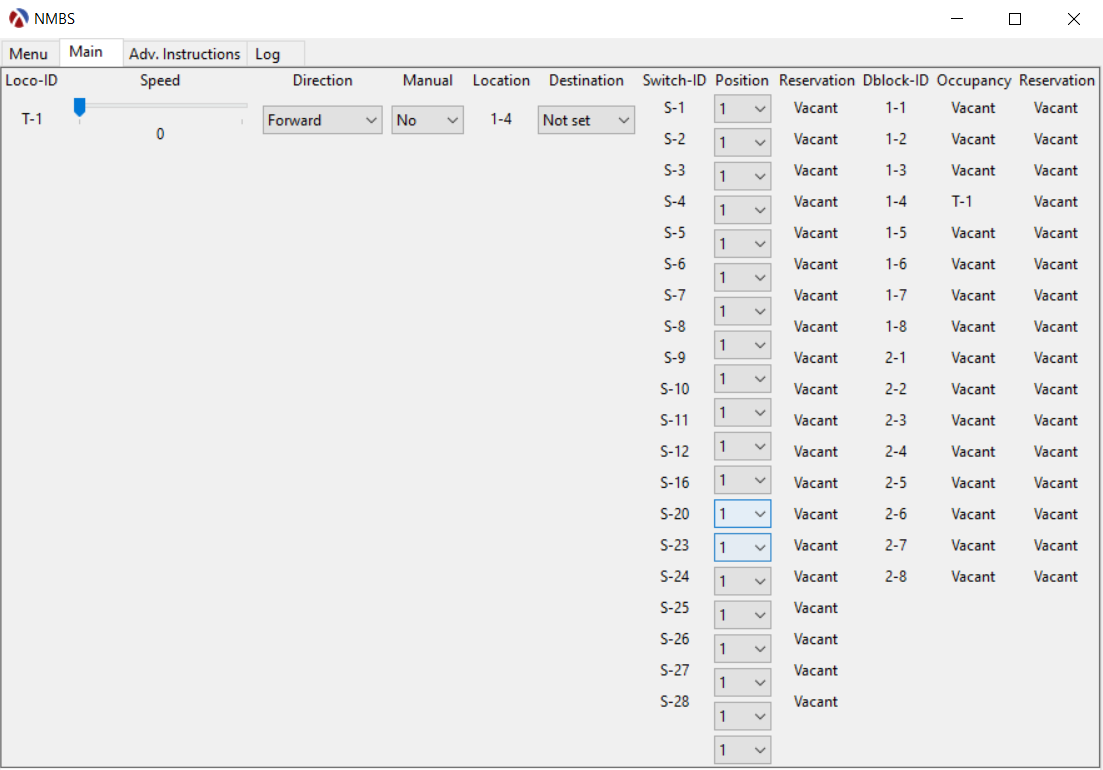
\includegraphics[width=\textwidth]{Images/Screenshot_5.png}
    \caption{De main tabblad.}
\end{figure}
\\
De functionaliteiten zijn opgedeelt in kolommen. In de eerste kolom zien we de ID van de locomotieven. In de 2e kolom hebben we een slider 
om te kunnen interageren met de snelheid met de locomotief. Vervolgens hebben we 2 choice boxes om de richting en reservatieprotocol te veranderen.
Het verschil in de reservatieprotocollen is dat als manueel aangeduid is dat het zal negeren dat er een trein een bepaalde
detectieblok bezet. Dit zal bijvoorbeeld gebruikt worden in het middeste gedeelte van de hardware setup modus. 
Vervolgens zien we de laatst geregistreerde locatie en dan krijgen we nog een optie het automatisch trajectbeheer in te schakelen met de gekozen eindbestemming.
Hierna hebben we het te maken met de wissels. De eerste kolom zal de ID weergeven en de tweede kolom zal interactie bieden met de wisselstand. De derde kolom zal de 
reservatiestatus geven van de wissels. De laatste 3 kolommen zijn analoog aan die van de wissels maar hierbij is er geen interactie mogelijk omdat deze geen wisselstand hebben
Het verschil is wel dat ze een bezettingstatus hebben die weergegeven wordt. 
\subsection{Adv. Instructions}
Dit tabblad zal het toevoegen en verwijderen van locomotieven aanbieden. In het gele kader kunnen we als eerste
de ID van de locomotief zetten gevolgd door de vorige locatie van de locomotief (let op: Dit moet een detectieblok zijn) en de huidige locatie.
Dit moet ook een detectieblok zijn. Nadat dit ingevuld is kunnen we op "ADD`` drukken. In het blauwe kader kunnen we de ID van de locomotief die we wensen te verwijderen invullen. 
Om de locomotief dan te verwijderen moeten we op "remove`` drukken. In het oranje kader zal alleen de ID van de bestaande locomotieven staan en parallel in het rode kader
zal de route weergegeven worden indien het automatisch trajectbeheer ingeschakeld is.  
\begin{figure}[h]
    \centering
    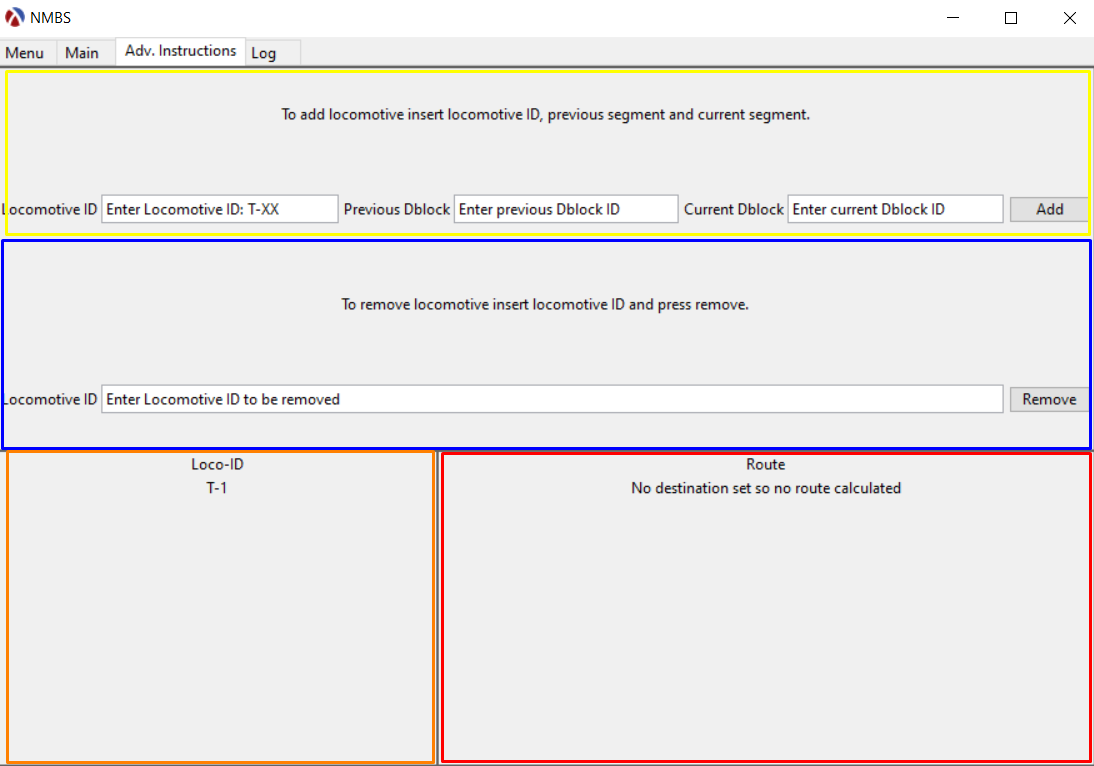
\includegraphics[width=\textwidth]{Images/Screenshot_6.png}
    \caption{De Adv. Instructions tabblad.}
\end{figure}
\subsection{Log}
In dit tabblad zullen de wijzigingen in het spoornetwerk weergegeven worden. Dit zullen bijvoorbeeld snelheid wijzigingen zijn of wisselstand wijzigingen. Hier is geen
interactie mee mogelijk maar dient om te zien wat er allemaal is uitgevoerd door infrabel. 
\end{document}